
\section{Ensemble de données}
\paragraph{}
Afin de développer le module d'apprentissage automatique mentionné précédemment (voir \ref{ProlemSolver}), nous avons choisis le data-set\footnote{Ensemble de données d'apprentissage} disponible dans \cite{dataset}, il s'agira donc d'analyser ces données(\ref{dataAnalysis}), de les pré-traiter éventuellement afin de les préparer pour la session d'apprentissage (\ref{learningSession})
\subsection{Description des données}
\paragraph{}
Comme expliqué dans \cite{datasetDetails}, les données d'apprentissage on été récupérées à l'aide de l'application Vicon-Tracker \cite{vico} ainsi que celle de marqueurs(au total de 11) placés sur la face arrière d'un gant, ces derniers servent de source de données envoyée à des capteurs positionnés sur les deux flancs(pour calculer la profondeur), la figure suivante illustre le procédé : 
\begin{minipage}{0.5\linewidth}
	\begin{figure}[H]
		\centering
		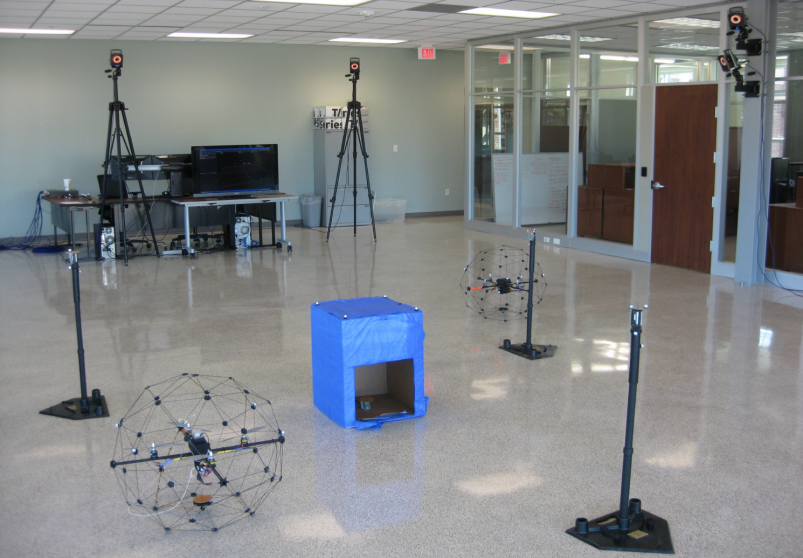
\includegraphics[width=\linewidth]{images/cameras.png}
		\caption{\small Environement ou les données on été capturées \cite{datasetDetails}}
	\end{figure}
\end{minipage}
\begin{minipage}{0.5\linewidth}
	\begin{figure}[H]
		\centering
		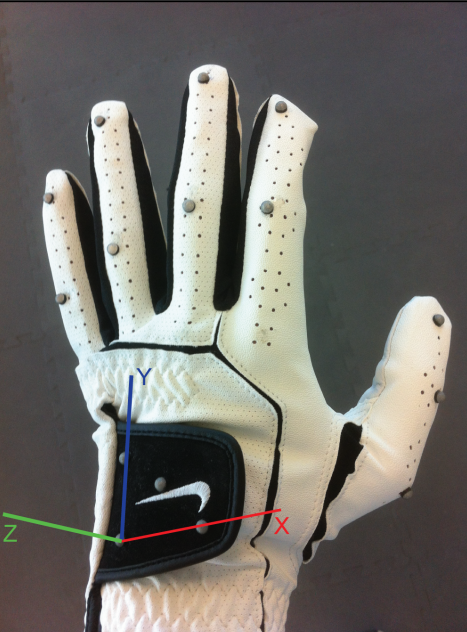
\includegraphics[width=0.5\linewidth]{images/glove.png}
		\caption{\small  Le gant utilisé pour y attaché les marqueurs( la source des données ) \cite{datasetDetails}}
	\end{figure}
\end{minipage}
\par 
Dans \cite{dataset}, on peut notamment trouvé une brève description des données brutes, elles sont sous forme d'un fichier \textbf{.csv} avec le délimiteur de cellules \textbf{,} (virgule), l'entête est structurée  de la manière suivante :
\begin{itemize}
	\item Les deux premières colonnes Class/User représentent répsectivement l'identifiant du geste observé (1 à 5) et l'identifiant de l'utilisateur(cobaye) qui a porté le gant durant cette session de collecte de données.
	\item Les 36 colonnes suivantes contiennent des nombres réels qui représentent les coordonnées cartésiennes en 3-dimensions $(x_i,y_i,z_i)$ des différents marqueurs $Marker_i$. \par Il est a noté d'après \cite{datasetDetails} et \cite{dataset} que les marqueurs sont non-étiquetés, c'est à dire que pour deux instances $I_1 et I_2$ du data-set, les coordonnés $(x_i^{I_1},y_i^{I_1},z_i^{I_1})$ et $(x_i^{I_2},y_i^{I_2},z_i^{I_2})$ ne désignent pas toujours les coordonnées du même marqueur $i$. \par En raison des conditions de captage des données certaines instances ont des données manquantes représentées par \textbf{?}
	\item Il est aussi mentionné dans \cite{datasetDetails} qu'au cours des séances de captage des données, certains objets qui ne sont pas des marqueurs on été captés par les capteurs, en conséquent un (ou plusieurs)marqueur(s) en plus a(ont) été(s) ajouté(s) par erreur aux données, il peut être donc considéré comme un bruit.\label{noise}
\end{itemize}
\subsection{Analyse et prétraitement des données}\label{dataAnalysis}
\paragraph{}
Une étape primordiale avant de se lancer dans les essaies d'apprentissage est l'analyse et la codification des données, nous avons d'abord effectué une analyse manuelle pour essayer de comprendre comment les données variaient, en nous inspirant des remarques faites dans \cite{datasetDetails} nous avons remarqué que durant l'enregistrent de la position des marqueurs, certains d'entre eux ne devenait plus visibles par les capteurs, fortement causé par la nature du geste et non pas a cause d'éventuelles perturbations, pour nous en assurer nous avons dresser le tableau suivant : 
\begin{table}[H]
	\centering
	\begin{tabular}{cc|c|c|c|c|c|c|c|c|c|}
		\cline{3-11}
		&           & \multicolumn{9}{c|}{Minimum number of Markers}                     \\ \cline{3-11} 
		& \textbf{}     & 4     & 5     & 6     & 7     & 8     & 9     & 10    & 11 & 12\\ \hline
		\multicolumn{1}{|c|}{\multirow{5}{*}{Gestures}} & 1         & 15604 & 14190 & 9191  & 2639  & 52    & 48    & 48    & 48    & 0  \\ \cline{2-11} 
		\multicolumn{1}{|c|}{}                          & 2         & 14978 & 14950 & 14909 & 14761 & 14668 & 14550 & 13524 & 10524 & 31 \\ \cline{2-11} 
		\multicolumn{1}{|c|}{}                          & 3         & 16322 & 15380 & 10746 & 6423  & 3556  & 81    & 0     & 0     & 0  \\ \cline{2-11} 
		\multicolumn{1}{|c|}{}                          & 4         & 14774 & 14769 & 14578 & 13018 & 5767  & 2349  & 13    & 0     & 0  \\ \cline{2-11} 
		\multicolumn{1}{|c|}{}                          & 5         & 15727 & 15686 & 15648 & 15406 & 14900 & 13535 & 10382 & 4180  & 0  \\ \hline
	\end{tabular}
	\caption{Nombre d'instances par classe de geste dont le nombre minimum de marqueurs est visible ( donnée non manquante dans le data-set)}
	\label{my-label}
\end{table}
\par 
Nous pouvons observer que par exemple, pour le geste 2 \textbf{tous les doigts levés} chaque instance étiquetée par cette classe possède tout les marqueurs visible à l'exception du dernier(Ce marqueur est très probablement le marqueurs en plus mentionné dans \ref{noise}), il en est presque de même pour le geste 5 \textbf{(geste de saisie un sorte de poing ouvert légèrement)}, nous pouvons voir que qu'il y a une petite différence avec les données de la classe 2, cela est du au fait que les marqueurs placés aux ongles ne sont pas toujours visibles.\par 
Pour le reste des classes, la classe 3 et 4 diffèrent en un seul marqueurs ou deux car les deux sont très similaires( \textbf{3} : un doigt levé, \textbf{4} : deux doigts levés), enfin pour les geste de la classe 1 \textbf{(Poing fermé)} le manque apparent de marqueurs visibles est expliqué par le fait que les marqueurs au jointure et extrémité des doigts soient masqués par la nature du geste en lui même.\par 
Bien que les valeurs manquantes ont une grande signification pour nous humains, il faut tout de même traduire cette information pour le modèle, deux approches ont été pensée.
\subsubsection{Approche naïve}\label{naiveApproache}
\paragraph{}
Affecter une(des) valeur(es) aux données manquantes est une tâche souvent ardue, une multitude de théories existent sur le sujet, mais parfois la solution la plus simple semble être la plus efficace, nous avons simplement remplacé le valeurs manquantes par des \textbf{zéros}, ce choix est appuyé par un raisonnement fait à partir de l'analyse faite préalablement, en effet chaque classe de geste suit un certain motif(pattern) de valeurs manquantes, autrement dit si nous devions remplacer ses valeurs manquante par une approximation(une moyenne sur les valeurs de la colonne par exemple) cela pourrait rapprocher les instances entre elles et donc pourrait fausser l'apprentissage, car les valeurs des attributs seraient trop proches l'une d'entre elles, les remplacer par une valeur nulle pourra en théorie aider le modèle a mieux distinguer les classes, pour ainsi mieux approximer le pattern que suivent ces données.\\
Cependant, le pattern résultant d’un tel remplacement de données dépend surtout de la méthode dont les données ont été collectées. Comme expliqué précédemment, les données manquantes sont dû au fait que la méthode utilisée pour les collecter ne détectait pas tous les marqueurs, certains gestes éclipsaient certains marqueurs, d’où le pattern de données manquantes.	
\subsubsection{Approche par Clustering}\label{clusterApproache}
\paragraph{}
L’approche par cluster essaye de minimiser la dépendance entre les données et la méthode avec la quelle elles sont collectées.\ref{my-label} L’idée c’est d’appliquer une sorte d’étiquetage de marqueurs en regroupant les coordonnées susceptibles d’appartenir au même marqueur dans un cluster. Nous avons utilisé un modèle de main 3D pour simuler les cinq gestes et collecter les coordonnées des marqueurs étiquetés.\\
\begin{center}
	\begin{figure}[H]
		\centering
		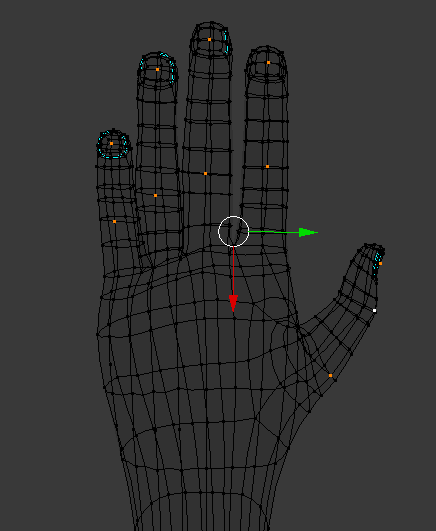
\includegraphics[scale=0.4]{images/3DModel.png}
		\caption{\small Modèle de main 3D avec marqueurs étiquetés}
	\end{figure}
\end{center}
L’ensemble des données est ensuite parcourue en affectant chaque point $(x_i,y_i,z_i)$ au marqueur le plus proche (voir \cite{knn} et \cite{knn2}) .\\
Le modèle 3D n’étant pas très fiable, ainsi que la différence entre les mains des utilisateurs génèrent un nombre important de collision, c’est à dire plusieurs point sont affectés au même marqueur. Pour y remédier, à l’affectation d’un point à un marqueur si ce dernier est déjà pris, on affecte le point au prochain marqueur le plus proche.\\
Évidemment à l’arriver d’une nouvelle donnée, soit en utilisant la même méthode de collection de données que le data-set d’apprentissage ou bien une autre méthode, le même traitement est effectué afin que cette donnée devienne conforme avec ceux qu’on génère en utilisant cette approche.